%%%%%%%%%%%%%%%%%%%%%%%%%%%%%%%%%%%%%%%%%%%%%%%%%%%%%%%%%%%%
%%  This Beamer template was created by Cameron Bracken.
%%  Anyone can freely use or modify it for any purpose
%%  without attribution.
%%
%%  Last Modified: January 9, 2009
%%

\documentclass[xcolor=x11names,compress]{beamer}

%% General document %%%%%%%%%%%%%%%%%%%%%%%%%%%%%%%%%%
\usepackage{graphicx}
\usepackage{tikz}
\usetikzlibrary{decorations.fractals}
%%%%%%%%%%%%%%%%%%%%%%%%%%%%%%%%%%%%%%%%%%%%%%%%%%%%%%


%% Beamer Layout %%%%%%%%%%%%%%%%%%%%%%%%%%%%%%%%%%
\useoutertheme[subsection=false,shadow]{miniframes}
\useinnertheme{default}
\usefonttheme{serif}
\usepackage{palatino}
\usepackage{epstopdf}
\usepackage[T1]{fontenc}
\usepackage[latin9]{inputenc}
\usepackage{array}
\usepackage{verbatim}
\usepackage{url}
\usepackage{multirow}
\usepackage{graphicx}
\PassOptionsToPackage{normalem}{ulem}
\usepackage{ulem}
\usepackage{epstopdf}
\usepackage{subfigure}
%\usepackage{algorithmic}
\DeclareMathOperator*{\argmax}{arg\,max}


\setbeamerfont{title like}{shape=\scshape}
\setbeamerfont{frametitle}{shape=\scshape}

\setbeamercolor*{lower separation line head}{bg=DeepSkyBlue4} 
\setbeamercolor*{normal text}{fg=black,bg=white} 
\setbeamercolor*{alerted text}{fg=red} 
\setbeamercolor*{example text}{fg=black} 
\setbeamercolor*{structure}{fg=black} 
 
\setbeamercolor*{palette tertiary}{fg=black,bg=black!10} 
\setbeamercolor*{palette quaternary}{fg=black,bg=black!10} 

\renewcommand{\(}{\begin{columns}}
\renewcommand{\)}{\end{columns}}
\newcommand{\<}[1]{\begin{column}{#1}}
\renewcommand{\>}{\end{column}}
%%%%%%%%%%%%%%%%%%%%%%%%%%%%%%%%%%%%%%%%%%%%%%%%%%

\begin{document}


\begin{frame}
\title{A Study of Query Reformulation for Patent Prior Art Search with Partial Patent Applications}
%\subtitle{SUBTITLE}
\author{
	Mohamed Reda Bouadjenek \\
	\textbf{Gabriela Ferraro}\\
	Scott Sanner\\
	%{\it Humboldt State University}\\
}
\date{
	\begin{tikzpicture}[decoration=Koch curve type 2] 
		\draw[DeepSkyBlue4] decorate{ decorate{ decorate{ (0,0) -- (3,0) }}}; 
	\end{tikzpicture}  
	\\
	\vspace{1cm}
	\today
}
\titlepage
\end{frame}


\begin{frame}
\frametitle{Outline}
\begin{itemize}
\item[-] Prior art search
\item[-] Query reformulation for patents
\item[-] General Query reformulation methods
\item[-]  
\item[-] Experiments 
\item[-] Results and discussion
\item[-] Conclusion and future work
\end{itemize}
\end{frame}

\section{\scshape Patent Prior Art Search with Partial Patent Applications}

\begin{frame}
\frametitle{What patents are?}

Patents are legal documents to protect an invention.

\begin{itemize}
\item[-] \textbf{Rich meta}: Inventor, Author, Company, Country, Publication year, etc.
\item[-] \textbf{Predefined document structure}: Title, Abstract, Description, Claims.		
\item[]
\end{itemize}

\begin{center}
\textbf{Patent Applications} vs. \textbf{Granted Patents}
\end{center}

\end{frame}


\begin{frame}
\frametitle{What is patent prior art search?}
{\color{DeepSkyBlue4}\textit{\textbf{Finding previously granted patents relevant for a patent application}}}

\begin{itemize}
\item[-] Patent examiners
\item[-] Patent authors/inventors
\end{itemize}


Challenges and data sets:
\begin{itemize}
\item NTCIR (since 2002)
\item TREC-Chem (2007)
\item CLEF-IP (2010/2011)*
\end{itemize}
\end{frame}



\begin{frame}
\frametitle{Patent Prior Art Search}
\begin{itemize}
\item[] Why patent prior art search is different to standard Information Retrieval (IR)?
  \begin{itemize}
  \item[]
  \item[-] \textbf{Queries} are full patent applications (hundreds of words organized into several sections)  	
   \item[]
  \item[-] \textbf{Recall-oriented} task (retrieve all relevant documents at early ranks)
  	while text and web search are \textbf{precision-oriented} (retrieve a subset of relevant documents)
  \end{itemize}
\end{itemize}
\end{frame}



\begin{frame}
\frametitle{Patent Prior Art Search with partial applications}
Writing a full patent application is time-consuming and costly

\begin{itemize}
\item[-] We proposed to do patent prior art search with \textbf{partial (incomplete) patent applications}
\item[-] Intensive study about query reformulation for patent prior art search with partial patent applications
\end{itemize}
\end{frame}


\begin{frame}
\frametitle{Querying with partial patent applications}

\begin{tiny}
\begin{itemize}
\item Term overlap (Jaccard Coefficient) of (ir)relevant documents with the result sets for different queries
\item Top 100 and bottom 100 queries
\item Top 10 irrelevant documents ranked by BM25 ~\cite{Robertson1993}
% (100 queries that perform the best, and 100 queries that perform the worst)
\item CLEP-IP 2010  
\end{itemize}
\end{tiny}

\begin{small}
\begin{figure}
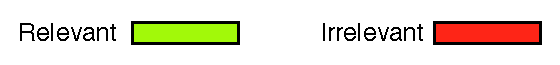
\includegraphics[width=3.5cm]{../img/legend} 

\subfigure[Title query]{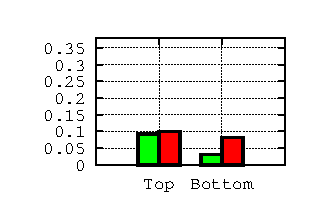
\includegraphics[width=2.5cm]{../Results-CIKM2014/jaccard-qTitle-CLEF-IP2010}}\subfigure[Abs. query]{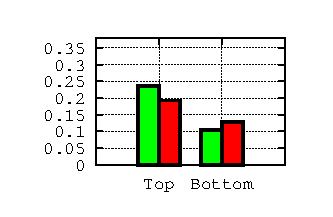
\includegraphics[width=2.5cm]{../Results-CIKM2014/jaccard-qAbstract-CLEF-IP2010}}\subfigure[Claims query]{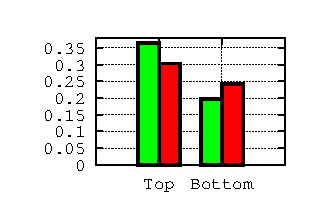
\includegraphics[width=2.5cm]{../Results-CIKM2014/jaccard-qClaims-CLEF-IP2010}}\subfigure[Desc. query]{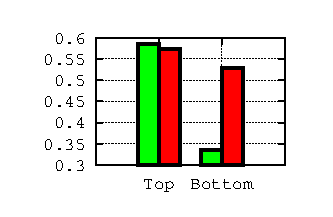
\includegraphics[width=2.5cm]{../Results-CIKM2014/jaccard-qDescription-CLEF-IP2010}}
\end{figure}
\end{small}
\end{frame}


\begin{frame}
\frametitle{Querying with partial patent applications}
There are 3 notable trends:
\begin{itemize}
\item[(i)]   term overlap increases from \textit{title} to \textit{description}
since the query size grows accordingly; 
\item[(ii)]  the bottom 100 performing queries tend to have much smaller term overlap with the relevant documents than the top 100 queries; 
\item[(iii)] the best overlap for any relevant
document set for any set of queries is less than one in four terms.
\end{itemize}

\begin{center}
{\color{DeepSkyBlue4}\textbf{We investigate Query Reformulation methods}}
\end{center}
\end{frame}



\begin{frame}
\frametitle{Query Reformulation}

{\color{DeepSkyBlue4}\textit{\textbf{Query reformulation} is the process of transforming an initial query $Q$ to another query $Q'$.}}

\begin{itemize}
\item \textbf{Query Reduction} (QR) \cite{Kumaran2009}: reduces the query such that superfluous information is removed.
\item \textbf{Query Expansion} (QE) \cite{Efthimiadis1996}: enhance the query with additional terms likely to occur in relevant documents.
\end{itemize}

%Intensive study about query reformulation for patent prior art search with partial patent applications
\end{frame}



\begin{frame}
\frametitle{Query Reformulation for patents}

\begin{itemize}
\item {\color{DeepSkyBlue4}\textbf{Query type}}: title, abstract, claims, description.

{\small \textit{\texttt{What part of a partial application an inventor
should write to obtain the best search results?}}}

\item {\color{DeepSkyBlue4}\textbf{Relevance model}}: BM25, vector space model (VSM): TF-IDF~\cite{Salton1975}
%For initial retrieval of documents in the \emph{pseudo-relevant} feedback set (PRF) and subsequent re-retrieval, a probabilistic approach represented by the popular BM25~\cite{Robertson1993} and vector space model (VSM) approach, TF-IDF~\cite{Salton1975}. 

{\small \textit{\texttt{Which relevance model works best for query reformulation
for patent prior art search? }}}

\item {\color{DeepSkyBlue4}\textbf{Query expansion source}}:  title, abstract,
claims, description
{\small \texttt{\textit{Are the title words of particularly high value as expansion terms? }}}
%* QE only

\item {\color{DeepSkyBlue4}\textbf{Term selection method}}: Rocchio~\cite{Salton1971}, 
MRRQR 
%new term selection methods that we propose in the next sections

{\small \textit{\texttt{Which is the best selection method? and with which query type, retrieval model, and term source? }}}
\end{itemize}
\end{frame}


\begin{frame}
\frametitle{Query Expansion (QE) Frameworks}

{\color{DeepSkyBlue4}\textit{QE aims to alleviate the term mi mismatch between queries an relevant documents.}}

\textbf{Rocchio} 

Derives a score for each potential query expansion term and in practice, the top-$k$ scoring terms (often for $k\ll200$) are used to expand the query and are
weighted according to their Rocchio score during the second stage
of retrieval. 
%The caveat of this approach is that given a limited budget of $k$ expansion terms, there is no inherent guarantee that these terms ``cover'' all documents in the pseudo-relevant set.

\textit{What is missed in Rocchio?}
\end{frame}



\begin{frame}
\frametitle{Diverse term selection}
\emph{Maximal Marginal Relevance} (MMR), a result set diversification algorithm  (MMR)~\cite{Carbonell1998}, usually used for \textbf{diverse document selection} (e.g., multi-document summarization) 
\end{frame}


\begin{frame}
\frametitle{Notation used in MMR QE/QR}

\begin{figure}
\begin{center}
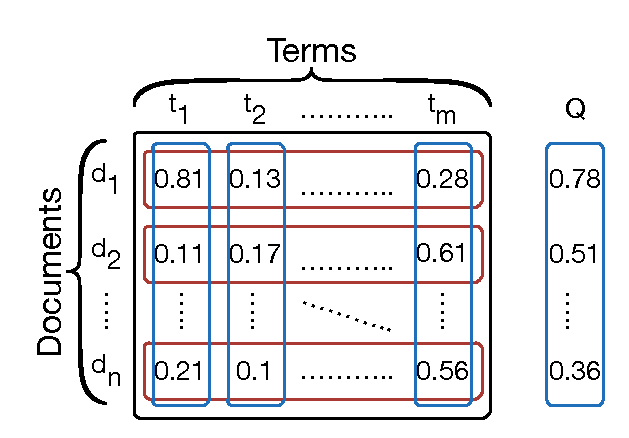
\includegraphics[width=5.5cm]{../img/matrix} 
\par\end{center}
\vspace{-1mm}
\label{fig:notation} 
\end{figure}

\begin{equation}
t_{k}^{*}=\argmax_{t_{k}\notin T_{k-1}^{*}}\hspace{-0.3mm}[\lambda\cos(Q,t_{k})-\hspace{-0.3mm}(1-\lambda)\max_{t_{j}\in T_{k-1}^{*}}\cos(t_{j},t_{k})]
\end{equation}


% We begin our formal description of MMRQE by first defining some necessary notation. MMRQE takes as input a pseudo-relevant feedback set of $n$ documents (PRF), which is obtained after a retrieval for the initial query. From the PRF set, we build a document-term matrix of $n$ documents and $m$ terms as shown in Figure~\ref{fig:notation}, which uses a TF-IDF weighting for each document vector (row $d_{i}$ for $1\leq i\leq n$). However, as we will see shortly, the view that will be important for us in this work is instead the term vector (column $t_{j}$ for $1\leq j\leq m$). To represent the query $Q$ column vector in Figure~\ref{fig:notation} having a numerical entry for every document $d_{i}$, we found that computing the BM25 or TF-IDF score between each document $d_{i}$ and the query provided the best performance (in our experiments, the score used is given by the indicated relevance model).

% Given a query representation $Q$, we aim to select an optimal subset of $k$ terms $T_{k}^{*}\subset D$ (where $|T_{k}^{*}|=k$ and $k\ll|m|$) relevant to $Q$ but inherently different from each other (i.e., diverse). This can be achieved by building $T_{k}^{*}$ in a greedy manner by choosing the next optimal term $t_{k}^{*}$ given the previous set of optimal term selections $T_{k-1}^{*}=\{t_{1}^{*},\ldots,t_{k-1}^{*}\}$ (assuming $T_{0}^{*}=\emptyset$) using the MMR diverse selection criterion:

%Here, the first cosine similarity term measures relevance between the query $Q$ and possible expansion term $t_{k}$ while the second term penalizes the possible expansion term according to it's cosine similarity with any currently selected term in $T_{k-1}^{*}$. The parameter $\lambda\in[0,1]$ trades off relevance and diversity and we found $\lambda=0.5$ to generally provide the best results in our experiments on the CLEF-IP training dataset collection.

\end{frame}

% The key insight we want to conclude this section with is that MMRQE does not select expansion terms independently as in practical usage of Rocchio, but rather it selects terms that have uncorrelated usage patterns across documents, thus hopefully encouraging diverse term selection that covers more documents for a fixed expansion budget $k$ and ideally, higher recall.


\begin{frame}
\frametitle{Query Reduction Frameworks}

{\color{DeepSkyBlue4}\textit{QR aims to short long queries}}

\vspace{0.3cm}
We investigate the impact of QR methods when 
querying with long sections such as \textit{abstract}, \textit{claims} or \textit{description}.

\begin{figure}
\begin{center}
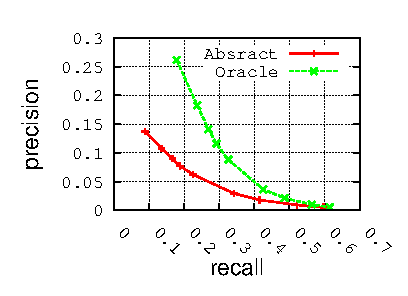
\includegraphics[width=4cm]{../analysis/precision-recall_ByField-CLEF-IP_2010}
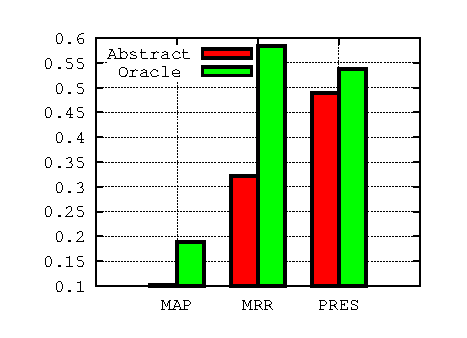
\includegraphics[width=4cm]{../analysis/MAP-MRR_ByField-CLEF-IP_2010}
\caption{Sample of terms removed from the abstract section}
\end{center}
\end{figure}

\begin{tiny}
\textbf{MAP}: Mean Average Precision;  \textbf{MRR}: Mean Reciprocal Rank; \textbf{PRES}: Patent Retrieval Evaluation Score
\end{tiny}
\end{frame}


\begin{frame}
\frametitle{The utility of query reduction for 1304 abstract queries of the CLEF-IP 2010 dataset}

\begin{tiny}
\begin{table}
\begin{centering}
%\caption{Sample of terms removed from the abstract section of CLEP-IP2010 Topic PAC-1019. }
\par\end{centering}

\begin{centering}
{\footnotesize{}}
\par\end{centering}{\footnotesize \par}

\centering{}{\scriptsize{}}%
\begin{tabular}{|l|c|c|c|c|c|}
\hline 
\multicolumn{6}{|>{\raggedright}p{8cm}|}{\textbf{\scriptsize{}Topic:}{\scriptsize{} PAC-1019}}\tabularnewline
\hline 
\multicolumn{6}{|>{\raggedright}p{8cm}|}{\textbf{\scriptsize{}Abstract:}{\scriptsize{} A 5-aminolevulinic acid
salt which is useful in fields of microorganisms, fermentation, animals,
medicaments, plants and the like; a process for producing the same;
a medical composition comprising the same; and a plant activator composition
comprising the same.}}\tabularnewline
\hline 
\hline 
\textbf{\scriptsize{}Term removed} & \textbf{\scriptsize{}P@5} & \textbf{\scriptsize{}P@10} & \textbf{\scriptsize{}R@10} & \textbf{\scriptsize{}AP} & \textbf{\scriptsize{}PRES}\tabularnewline
\hline 
{\scriptsize{}composit...} & \textbf{\scriptsize{}0.600} & {\scriptsize{}0.300} & {\scriptsize{}0.428} & \textbf{\scriptsize{}0.360} & \textbf{\scriptsize{}0.829}\tabularnewline
\hline 
{\scriptsize{}activ...} & {\scriptsize{}0.400} & {\scriptsize{}0.300} & {\scriptsize{}0.428} & {\scriptsize{}0.277} & \textbf{\scriptsize{}0.809}\tabularnewline
\hline 
{\scriptsize{}anim...} & \textbf{\scriptsize{}0.600} & {\scriptsize{}0.300} & {\scriptsize{}0.428} & \textbf{\scriptsize{}0.345} & \textbf{\scriptsize{}0.798}\tabularnewline
\hline 
{\scriptsize{}produc...} & {\scriptsize{}0.400} & {\scriptsize{}0.300} & {\scriptsize{}0.428} & \textbf{\scriptsize{}0.286} & \textbf{\scriptsize{}0.797}\tabularnewline
\hline 
{\scriptsize{}ferment...} & {\scriptsize{}0.200} & {\scriptsize{}0.300} & {\scriptsize{}0.428} & \textbf{\scriptsize{}0.283} & \textbf{\scriptsize{}0.796}\tabularnewline
\hline 
{\scriptsize{}microorgan...} & \textbf{\scriptsize{}0.600} & {\scriptsize{}0.300} & {\scriptsize{}0.428} & \textbf{\scriptsize{}0.333} & \textbf{\scriptsize{}0.793}\tabularnewline
\hline 
{\scriptsize{}compris...} & {\scriptsize{}0.400} & {\scriptsize{}0.300} & {\scriptsize{}0.428} & {\scriptsize{}0.271} & \textbf{\scriptsize{}0.790}\tabularnewline
\hline 
{\scriptsize{}medica...} & {\scriptsize{}0.400} & {\scriptsize{}0.300} & {\scriptsize{}0.428} & \textbf{\scriptsize{}0.297} & \textbf{\scriptsize{}0.789}\tabularnewline
\hline 
{\scriptsize{}medic...} & {\scriptsize{}0.400} & {\scriptsize{}0.300} & {\scriptsize{}0.428} & \textbf{\scriptsize{}0.297} & \textbf{\scriptsize{}0.787}\tabularnewline
\hline 
{\scriptsize{}field...} & {\scriptsize{}0.400} & {\scriptsize{}0.300} & {\scriptsize{}0.428} & \textbf{\scriptsize{}0.282} & \textbf{\scriptsize{}0.782}\tabularnewline
\hline 
{\scriptsize{}plant...} & {\scriptsize{}0.200} & {\scriptsize{}0.200} & {\scriptsize{}0.285} & {\scriptsize{}0.114} & {\scriptsize{}0.774}\tabularnewline
\hline 
{\scriptsize{}process...} & {\scriptsize{}0.400} & {\scriptsize{}0.300} & {\scriptsize{}0.428} & {\scriptsize{}0.279} & {\scriptsize{}0.764}\tabularnewline
\hline 
{\scriptsize{}acid...} & {\scriptsize{}0.400} & {\scriptsize{}0.300} & {\scriptsize{}0.428} & {\scriptsize{}0.252} & {\scriptsize{}0.693}\tabularnewline
\hline 
{\scriptsize{}salt...} & {\scriptsize{}0.200} & {\scriptsize{}0.200} & {\scriptsize{}0.285} & {\scriptsize{}0.216} & {\scriptsize{}0.663}\tabularnewline
\hline 
{\scriptsize{}aminolevulin...} & {\scriptsize{}0.000} & {\scriptsize{}0.100} & {\scriptsize{}0.142} & {\scriptsize{}0.026} & {\scriptsize{}0.352}\tabularnewline
\hline 
\hline 
\textbf{\scriptsize{}Baseline} & {\scriptsize{}0.400} & {\scriptsize{}0.300} & {\scriptsize{}0.428} & {\scriptsize{}0.280} & {\scriptsize{}0.777}\tabularnewline
\hline 
\end{tabular}
\end{table}
\end{tiny}

\end{frame}



\begin{frame}
\frametitle{Experiments Setup}
\begin{itemize}
\item CLEF-IP 2010: 
	\begin{itemize}
		\item 2.6 million patent documents
		\item 1303 English topics (queries)
	\end{itemize}
\item CLEF-IP 2011: 3 million patent documents
	\begin{itemize}
		\item 2.6 million patent documents
		\item 1351 English topics (queries)
	\end{itemize}
\item Lucene IR System
\item LucQE: Rocchio method for Lucene
\item Standard stop-words removal
\item Patent-specific stop-words removal \cite{Magdy2012}
\item Each patent section is indexed in a separate field
\item Queries target all the fields in the index
\item Filtering using the International patent Classification (IPC) of the queries \cite{Lopez2009,Roda2009}
\item Evaluation on the top 1000 results
\end{itemize}

%\footnote{We used the LucQE module, which provides an implementation of the Rocchio QE method for Lucene. \\ \texttt{http://lucene-qe.sourceforge.net/}%} to index the English subset of CLEF-IP 2010 and CLEF-IP 2010 datasets%\footnote{\texttt{\url{http://www.ifs.tuwien.ac.at/~clef-ip/}}%}~\cite{Piroi2011,Roda2009} with the default stemming and stop-word removal. We removed patent-specific stop-words as described in \cite{Magdy2012}. CLEF-IP 2010 contains 2.6 million patent documents and CLEF-IP 2011 consists of 3 million patent documents. The English test sets of CLEF-IP 2010 and CLEF-IP 2011 correspond to 1303 and 1351 topics respectively. In our implementation, each section of a patent (title, abstract,  claims, and description) is indexed in a separate field, so that different sections can be used, for example, as source of expansion terms. But, when a query is processed, all fields in the index are targeted, since it is sensible to use all available content. We also used the patent classification (IPC) for filtering the results by constraining them to have common classifications with the patent topic as suggested in previous works \cite{Lopez2009,Roda2009}. Finally, we report MAP, and PRES, which combines Recall with the quality of ranking and weights relevant documents lower in the ranking more highly than MAP. We report the evaluation metrics on the top 1000 results.
\end{frame}



\begin{frame}
\frametitle{Query Expansion Baselines}

\begin{itemize}
\item {\color{DeepSkyBlue4}General QE method}
	\begin{itemize}
	\item Rocchio \cite{}
	\end{itemize}
\item {\color{DeepSkyBlue4}Patent specific QE methods}
	\begin{itemize}
	\item \textbf{IPC} \cite{Mahdabi2013} used the text definitions of the  codes assigned to a patent application as a source for expansion.
	\item \textbf{WSynSet} \cite{Magdy2011} used the probability associated with the SynSet entries as a weight for each expanded term in the query.
	\item \textbf{USynSet} \cite{Magdy2011} used uniform weighting for all synonyms of a given term 
	\end{itemize}
\end{itemize}
	
% \cite{Magdy2011} generates candidate synonyms sets for terms, and use it as a source of expansion.  (i) used the probability associated with the SynSet entries as a weight for each expanded term in the query (\textbf{WSynSet}). Therefore, each term was replaced with its SynSet entries with the probability of each item in the SynSet acting as a weight to the term within the query.  
%(ii) used uniform weighting for all synonyms of a given term (\textbf{USynSet}).

%The combination of QE methods, relevance model and term selection options give us seven QE algorithms to evaluate.
% When MMRQE is used in combination with the VSM, the additional terms use the weights provided by the Rocchio method, whereas when using MMRQE and Rocchio with BM25, there is no need to weight the terms.

\begin{small}
* For all methods, their parameters were fixed to their optimal values,which were estimated using the CLEF-IP training queries.
\end{small}

\end{frame}


\begin{frame}
\frametitle{Other QE methods}

\begin{itemize}
\item Magdy et al. \cite{Magdy2011} classic techniques of query expansion: WordNet
%However, none of these approaches were able to achieve a significant improvement over the baseline/queries without expansion
\item Bashir et al. \cite{Bashir2010} with SRF set, used a machine learning approach by picking terms that may have a potential positive impact on the retrieval effectiveness. 

%However, this approach can be computational expensive, since the presented features are complicated to compute, which features??

\item Verma and Varma \cite{Verma2011}: used IPC codes as queries, which are expanded using the citation network. 
%The formed query is used to perform an initial search. The results are then re-ranked using queries constructed from patent text. Throughout our experiments,
%we concluded that relying on other terms to form a query rather than those in the patent application, leads to poor retrieval quality.  Therefore, the approach proposed in \cite{Verma2011} doesn't guarantee to obtain good performance. %
\end{itemize}

\end{frame}


\begin{frame}
\frametitle{Pseudo Relevant Feedback (PRF) size}

Effect of PRF set with various numbers of feedback documents on the CLEF-IP 2010 dataset. 

\begin{table}
\centering{}{\scriptsize{}}%
\begin{tabular}{|l|c|c|c|c|c|}
\hline 
\textbf{\scriptsize{}Query/Source} & \textbf{\scriptsize{}Metric} & \textbf{\scriptsize{}Method} & \textbf{\scriptsize{}5} & \textbf{\scriptsize{}10} & \textbf{\scriptsize{}20}\tabularnewline
\hline 
\hline 
{\scriptsize{}Query: Abstract} & {\scriptsize{}MAP} & {\scriptsize{}Rocchio} & {\scriptsize{}0.074} & {\scriptsize{}0.072} & {\scriptsize{}0.070}\tabularnewline
\cline{3-6} 
 & {\scriptsize{}BL=0.073} & {\scriptsize{}MMRQE} & {\scriptsize{}0.074} & {\scriptsize{}0.071} & {\scriptsize{}0.071}\tabularnewline
\cline{2-6} 
{\scriptsize{}Source: Claims} & {\scriptsize{}PRES} & {\scriptsize{}Rocchio} & {\scriptsize{}0.409} & {\scriptsize{}0.409} & {\scriptsize{}0.409}\tabularnewline
\cline{3-6} 
 & \multirow{1}{*}{{\scriptsize{}BL=0.403}} & {\scriptsize{}MMRQE} & {\scriptsize{}0.411} & {\scriptsize{}0.411} & {\scriptsize{}0.410}\tabularnewline
\hline 
{\scriptsize{}Query: Claims} & {\scriptsize{}MAP} & {\scriptsize{}Rocchio} & {\scriptsize{}0.083} & {\scriptsize{}0.080} & {\scriptsize{}0.079}\tabularnewline
\cline{3-6} 
 & {\scriptsize{}BL=0.081} & {\scriptsize{}MMRQE} & {\scriptsize{}0.082} & {\scriptsize{}0.080} & {\scriptsize{}0.080}\tabularnewline
\cline{2-6} 
{\scriptsize{}Source: Claims} & {\scriptsize{}PRES} & {\scriptsize{}Rocchio} & {\scriptsize{}0.443} & {\scriptsize{}0.445} & {\scriptsize{}0.446}\tabularnewline
\cline{3-6} 
 & {\scriptsize{}BL=0.433} & {\scriptsize{}MMRQE} & {\scriptsize{}0.445} & {\scriptsize{}0.444} & {\scriptsize{}0.442}\tabularnewline
\hline 
\end{tabular}
\end{table}

* 20 terms are used for query expansion
\end{frame}



\begin{frame}
\frametitle{Experiments for QE}

Experiments options:

\begin{itemize}
\item \textbf{\footnotesize{}Query type:}{\footnotesize{} $\{\mathrm{Title},\mathrm{Abstract},\mathrm{Claims},\mathrm{Description}\}$ }{\footnotesize \par}
\item \textbf{\footnotesize{}Query expansion source:}{\footnotesize{} $\{\mathrm{Title},\mathrm{Abstract},\mathrm{Claims},\mathrm{Description}\}$ }{\footnotesize \par}
\item \textbf{\footnotesize{}Relevance model:}{\footnotesize{} $\{\mathrm{BM25},\mbox{Vector-space Model}\}$ }{\footnotesize \par}
\item \textbf{\footnotesize{}Term selection method:}{\footnotesize{} $\{\mathrm{Rocchio},\mathrm{MMRQE},etc...\}$ }{\footnotesize \par}
\end{itemize}
\end{frame}




\begin{frame}
\frametitle{Experiements results for QE}

\textbf{Query}: Claims 

\textbf{Date set}: CLEF-IP 2010 

\textbf{Expansion source}: Abstract 

\begin{figure}
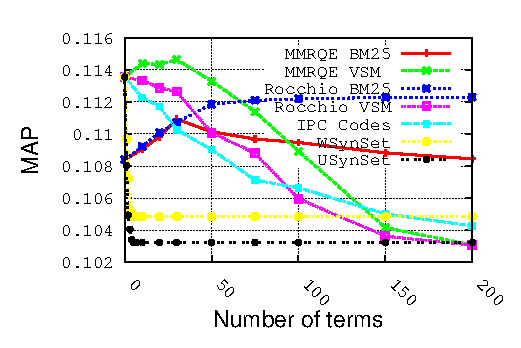
\includegraphics[width=6cm]{../Results-CIKM2014/qClaims-sAbstract_MAP_2010}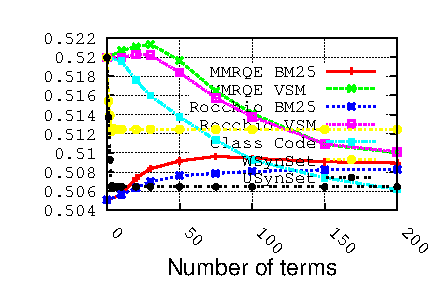
\includegraphics[width=6cm]{../Results-CIKM2014/qClaims-sAbstract_PRES_2010}
\end{figure}
\end{frame}



\begin{frame}
\frametitle{Samples of queries (CLEF-IP 2011) where QE improves
the performance}

%\begin{table}
%\caption{Samples of queries extracted from CLEF-IP 2011, where QE improves the performance (P: Precision, R: Recall, RR: Reciprocal Rank, AP:  Average Precision, PRES: Patent Retrieval Evaluation Score). MMRQE improves the two first examples, hile Rocchio improves the third. }
%\label{tbl:QESampleQueries}

\end{frame}



\begin{frame}
\frametitle{Query Reduction baselines}

\begin{itemize}
\item {\color{DeepSkyBlue4}General QR method}
	\begin{itemize}
	\item \textbf{RocchioQR} method for query pruning
%Basically, the idea is once we have computed the Rocchio modified query vector, we take only terms of the initial query that appear in this vector and rank them using the Rocchio score. Then, we remove $n$ terms with the lower score. We refer to this approach as \textbf{RocchioQR}.
	\end{itemize}	
\item {\color{DeepSkyBlue4}Patent specific methods}	
	\begin{itemize}
	\item \textbf{LMQR} \cite{Ganguly2011}: (i) computes Language Modeling similarities by calculating the probability of generating each segment from the top ranked documents; (ii) remove the least similar terms.
	\item \textbf{IPC}: 
	%(i) For each patent application, we take the definitions of the IPC codes which are associated to it. 
(i) rank the terms of the query according to both their frequency in the class
code definition, and their frequency in the query.
(ii) remove bottom terms of this ranking.
%(i.e. good terms are terms that occur a lot in the query, and few in the class code definition, whereas bad terms are those that occur few in the query, and a lot in the class code definition).  The intuition is that, terms in the IPC code definition may represent \textquotedbl{}stopwords\textquotedbl{}, especially if they are rare (infrequent in the patent application).
\end{itemize}
\end{itemize}

\vspace{0.5cm}
\begin{small}
{\color{DeepSkyBlue4}Other work}: \cite{Mahdabi2013} short queries by taking only the first claim of a patent application.
%This approach has not been implemented as its authors already point out its poor performance.
\end{small}
\end{frame}



\begin{frame}
\frametitle{QR discussion}
Best QR performance results are also obtained when using few
documents in the PRF set (top 5).
Impact of the diversity parameter $\lambda$ on the performance of
MMRQR on the CLEF-IP 2010 dataset
%Figure \ref{fig:DivImpactMMRQR} shows the impact of the diversity parameter $\lambda$ on the performance of MMRQR. The results are shown using BM25 retrieval model, and using abstract and claims for querying. Throughout our experiments, we concluded that the best value of $\lambda$ is 0.8, which indicates that few diversification in term selection can provide some improvement. It is clear that if we consider only diversification to select terms ($\lambda=0$), the ove rall performance are significantly degraded. This is certainly due to the fact that if we consider only diversified terms in the query, there is a loss in the meaning of the query, and thus, we increase the probability of retrieving irrelevant patents.

\begin{figure}
\begin{centering}
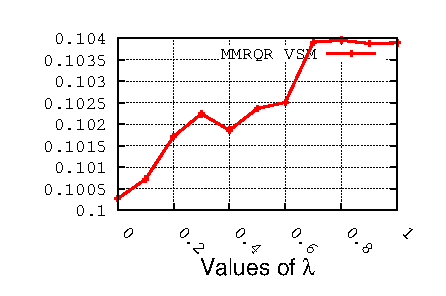
\includegraphics[width=4.3cm]{../mmrqrResults-lambda/qAbstract-sDescription_MAP_2010}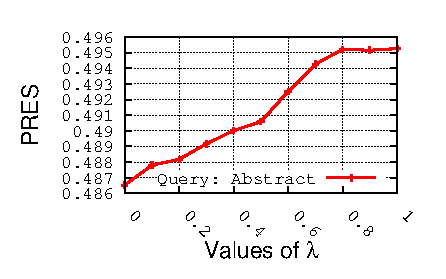
\includegraphics[width=4.3cm]{../mmrqrResults-lambda/qAbstract-sDescription_PRES_2010}
\par\end{centering}

\begin{centering}
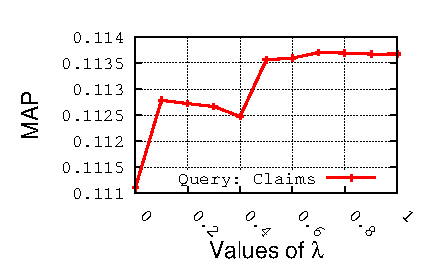
\includegraphics[width=4.3cm]{../mmrqrResults-lambda/qClaims-sDescription_MAP_2010}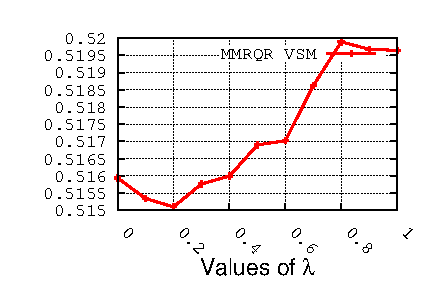
\includegraphics[width=4.3cm]{../mmrqrResults-lambda/qClaims-sDescription_PRES_2010}
\par\end{centering}
\end{figure}
\end{frame}



\begin{frame}
\frametitle{QR experiments}
Experiment options:
\begin{itemize}
\item \textbf{\footnotesize{}Query type:}{\footnotesize{} $\{\mathrm{Title},\mathrm{Abstract},\mathrm{Claims},\mathrm{Description}\}$ }{\footnotesize \par}
\item \textbf{\footnotesize{}Relevance model:}{\footnotesize{} $\{\mathrm{BM25},\mbox{Vector-space Model (VSM)}\}$ }{\footnotesize \par}
\item \textbf{\footnotesize{}Term selection method:}{\footnotesize{} $\{\mathrm{RocchioQR},\mathrm{MMRQR},etc...\}$ }{\footnotesize \par}
\end{itemize}
\end{frame}


\begin{frame}
\frametitle{Sample table!!!}
\end{frame}


\begin{frame}
\frametitle{QR while using the Description section for querying (CLEF-IP 2010)}

\begin{center}
\begin{figure}
\begin{centering}
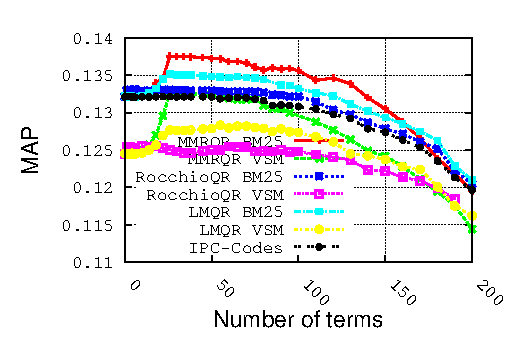
\includegraphics[width=4.3cm]{../mmrqrResults/qDescription-sDescription_MAP_2010}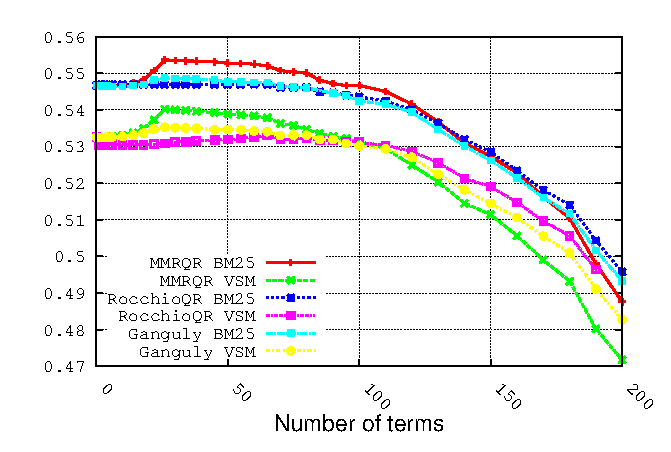
\includegraphics[width=4.3cm]{../mmrqrResults/qDescription-sDescription_PRES_2010}
\par\end{centering}
\end{figure}
\par\end{center}

\begin{small}
\begin{itemize}
\item (i) for VSM and BM25, MMRQE
provides the best performance for MAP and PRES (except for MAP,
where Rocchio BM25 provides better performance than MMRQE BM25);

\item (ii) adding more than 50 terms hurts the performance of MMRQE and Rocchio;

\item (iii) exploiting external sources provides poor performance (IPC code definition and SynSets). 
\end{itemize}
\end{small}

\end{frame}


\begin{frame}
\frametitle{MAP for QE methods on CLEF-IP 2010}
%Patent Retrieval Evaluation Score ( 

\begin{figure}
\begin{centering}
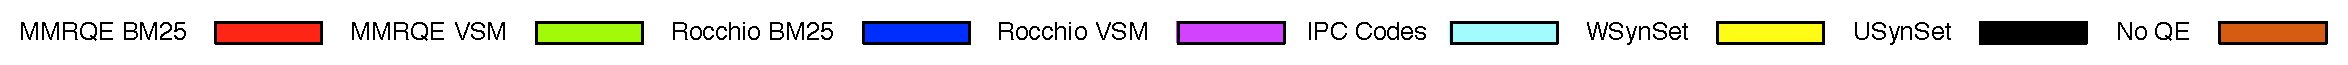
\includegraphics[width=10cm]{../img/legendQE}
\par\end{centering}

\begin{centering}
\subfigure[{\tiny Query Title.}]{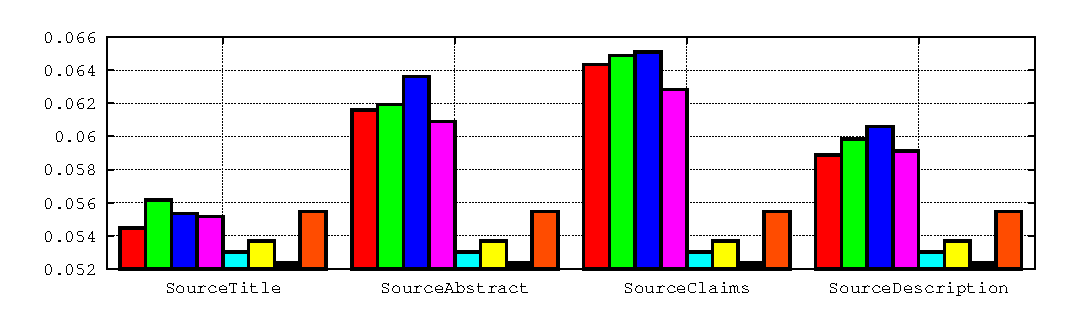
\includegraphics[width=5.5cm]{../Results-CIKM2014/qTitle-MAP-CLEF-IP2010}}\subfigure[{\tiny Query Abstract.}]{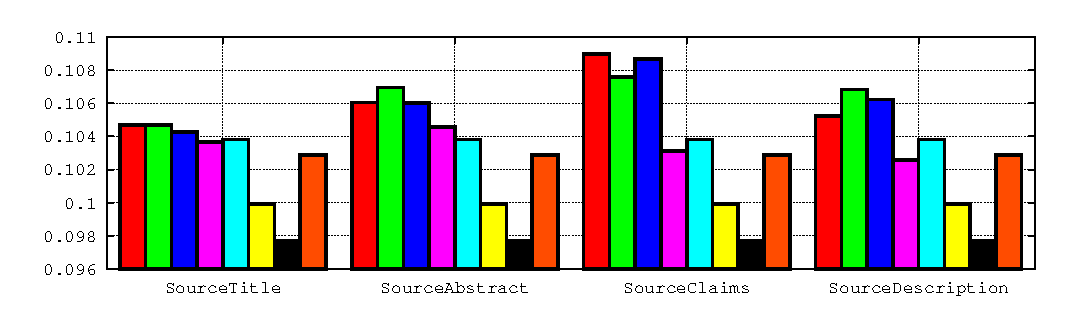
\includegraphics[width=5.5cm]{../Results-CIKM2014/qAbstract-MAP-CLEF-IP2010}}
\par\end{centering}

\begin{centering}
\subfigure[{\tiny Query Claims.}]{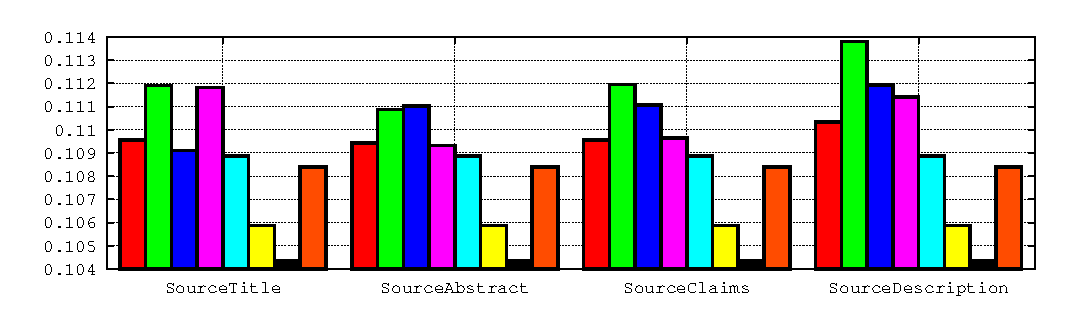
\includegraphics[width=5.5cm]{../Results-CIKM2014/qClaims-MAP-CLEF-IP2010}}\subfigure[{\tiny Query Description.}]{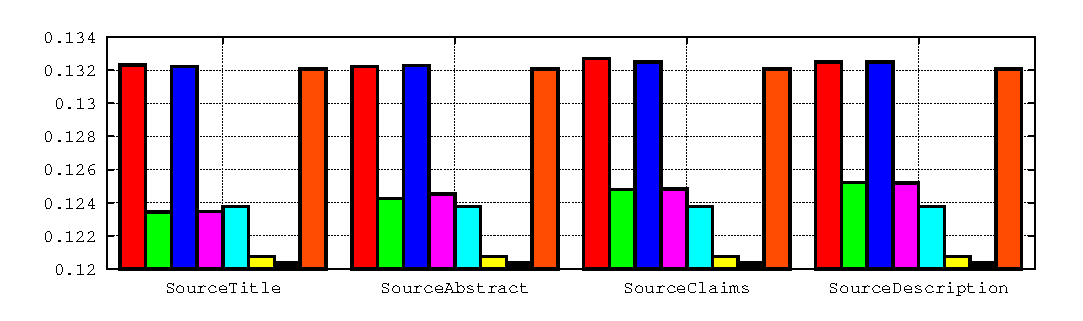
\includegraphics[width=5.5cm]{../Results-CIKM2014/qDescription-MAP-CLEF-IP2010}\label{fig:qDescription-MAP-CLEF-IP2010}}
\par\end{centering}
\end{figure}

{\small *for MMRQE $\lambda=0.5$}
\end{frame}

\begin{frame}
\frametitle{PRES for QE methods on CLEF-IP 2010}

\begin{figure}
\begin{centering}
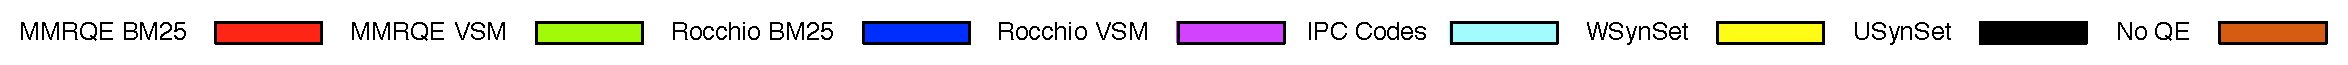
\includegraphics[width=10cm]{../img/legendQE}
\par\end{centering}

\begin{centering}
\subfigure[{\tiny Query Title.}]{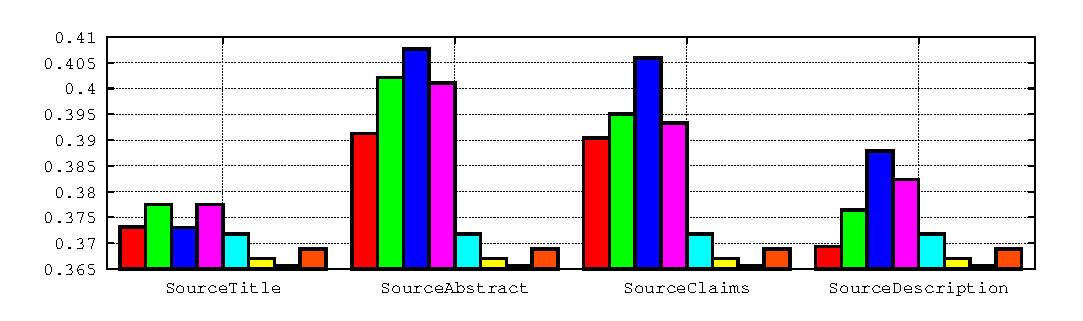
\includegraphics[width=5.5cm]{../Results-CIKM2014/qTitle-PRES-CLEF-IP2010}}\subfigure[{\tiny Query Abstract.}]{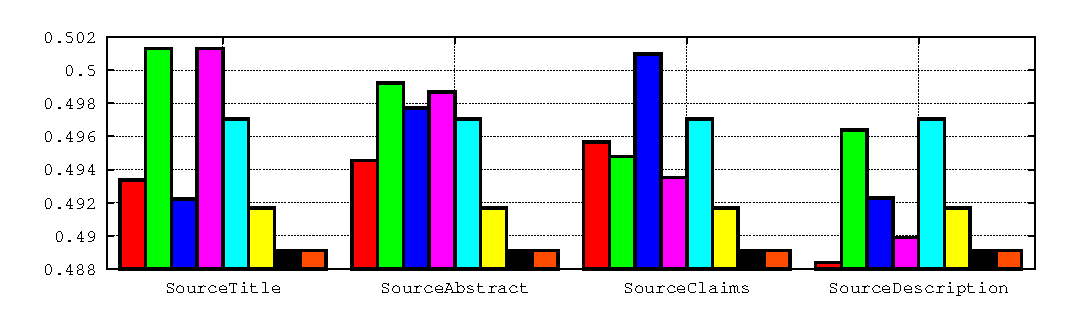
\includegraphics[width=5.5cm]{../Results-CIKM2014/qAbstract-PRES-CLEF-IP2010}}
\par\end{centering}

\begin{centering}
\subfigure[{\tiny Query Claims.}]{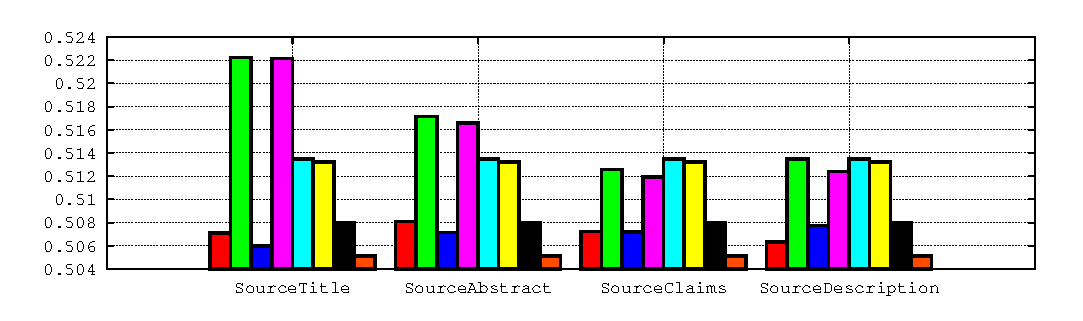
\includegraphics[width=5.5cm]{../Results-CIKM2014/qClaims-PRES-CLEF-IP2010}}\subfigure[{\tiny Query Description.}]{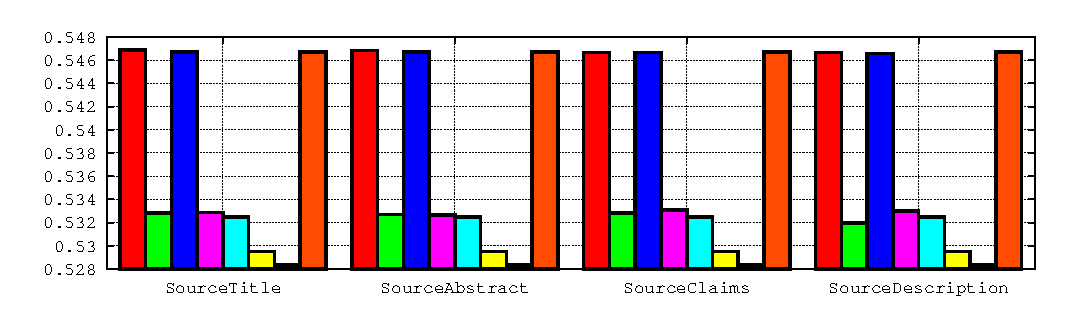
\includegraphics[width=5.5cm]{../Results-CIKM2014/qDescription-PRES-CLEF-IP2010}\label{fig:qDescription-PRES-CLEF-IP2010}} 
\par\end{centering}

{\small *for MMRQE $\lambda=0.5$}
%\caption{Patent Retrieval Evaluation Score (PRES) for QE methods on CLEF-IP 2010 (}
\end{figure}
\end{frame}


\begin{frame}
\frametitle{MAP for QE methods on CLEF 2011}

\begin{figure}
\begin{centering}
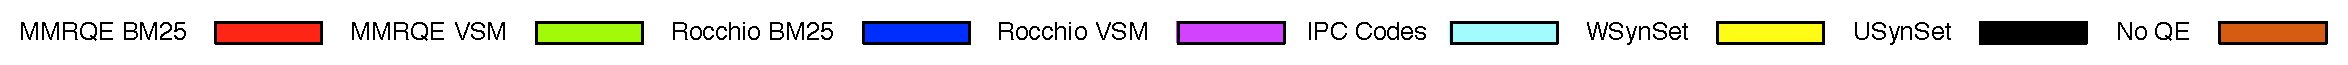
\includegraphics[width=10cm]{../img/legendQE}
\par\end{centering}

\begin{centering}
\subfigure[{\tiny Query Title.}]{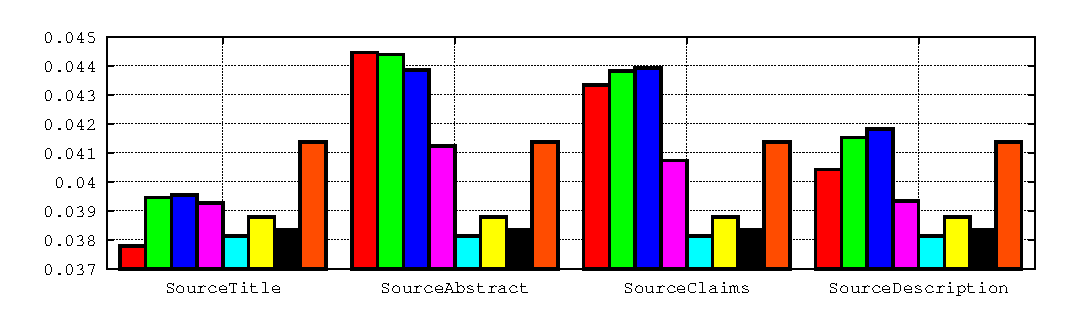
\includegraphics[width=5.5cm]{../Results-CIKM2014/qTitle-MAP-CLEF-IP2011}}\subfigure[{\tiny Query Abstract.}]{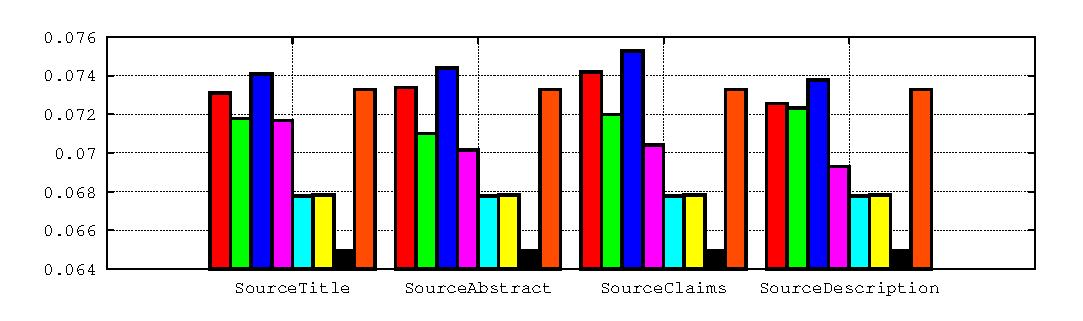
\includegraphics[width=5.5cm]{../Results-CIKM2014/qAbstract-MAP-CLEF-IP2011}}
\par\end{centering}

\begin{centering}
\subfigure[{\tiny Query Claims.}]{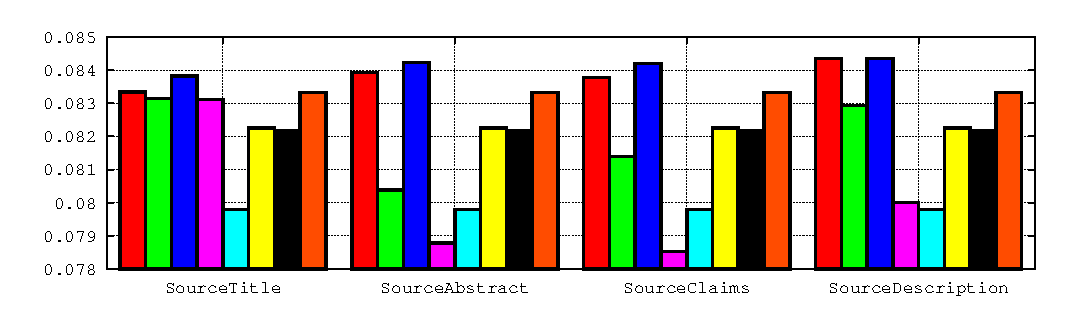
\includegraphics[width=5.5cm]{../Results-CIKM2014/qClaims-MAP-CLEF-IP2011}}\subfigure[{\tiny Query Description.}]{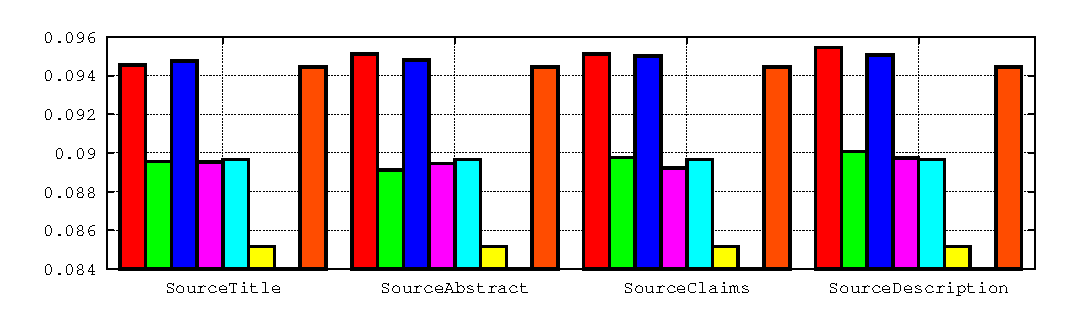
\includegraphics[width=5.5cm]{../Results-CIKM2014/qDescription-MAP-CLEF-IP2011}\label{fig:qDescription-MAP-CLEF-IP2011}} 
\par\end{centering}
%\caption{Mean Average Precision (MAP) for QE methods on CLEF-IP 2011 (for MMRQE $\lambda=0.5$).} \label{fig:MAP-CLEF2011}
\end{figure}
{\small *for MMRQE $\lambda=0.5$}
\end{frame}



\begin{frame}
\frametitle{PRES for QE methods on CLEF 2011}

\begin{figure}
\begin{centering}
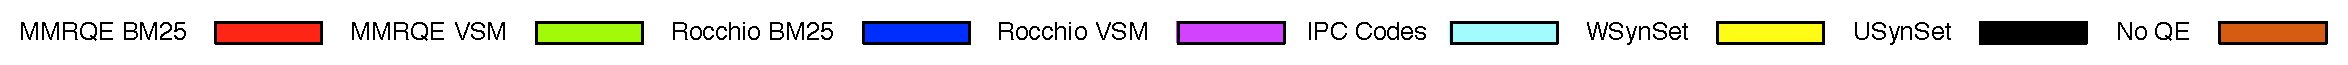
\includegraphics[width=10cm]{../img/legendQE}
\par\end{centering}

\begin{centering}
\subfigure[{\tiny Query Title.}]{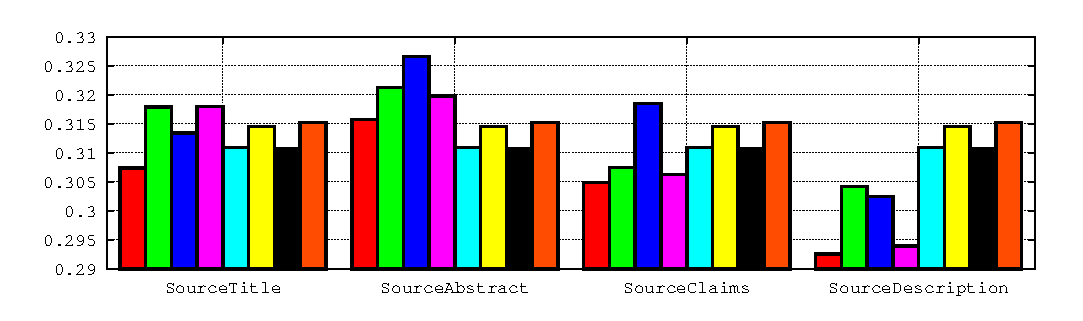
\includegraphics[width=5.5cm]{../Results-CIKM2014/qTitle-PRES-CLEF-IP2011}}\subfigure[{\tiny Query Abstract.}]{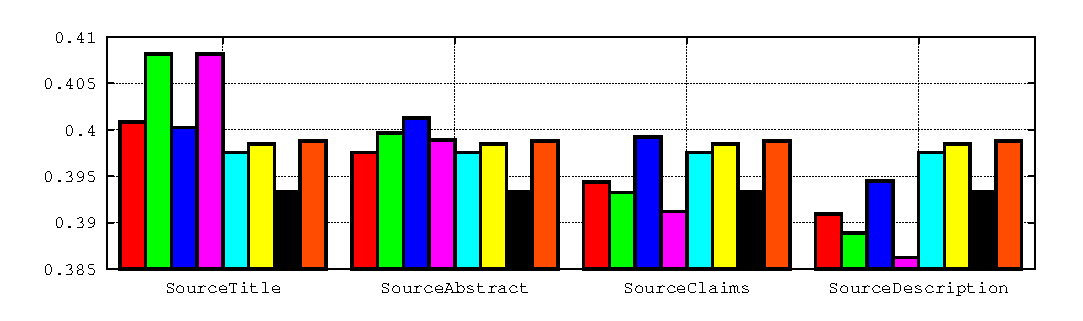
\includegraphics[width=5.5cm]{../Results-CIKM2014/qAbstract-PRES-CLEF-IP2011}}
\par\end{centering}

\begin{centering}
\subfigure[{\tiny Query Claims.}]{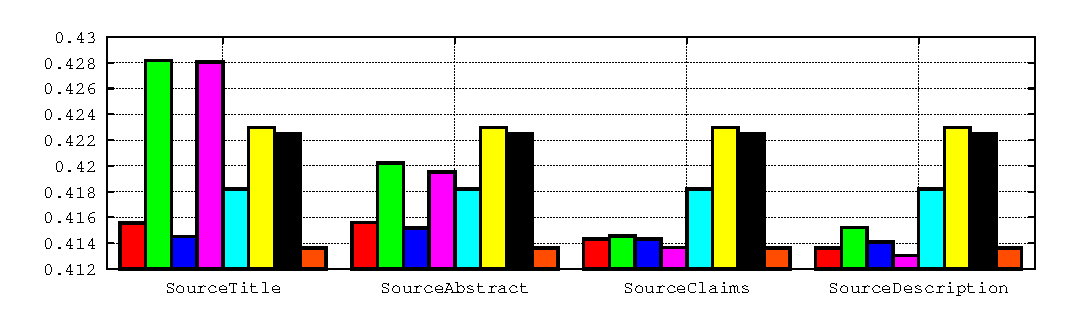
\includegraphics[width=5.5cm]{../Results-CIKM2014/qClaims-PRES-CLEF-IP2011}}\subfigure[{\tiny Query Description.}]{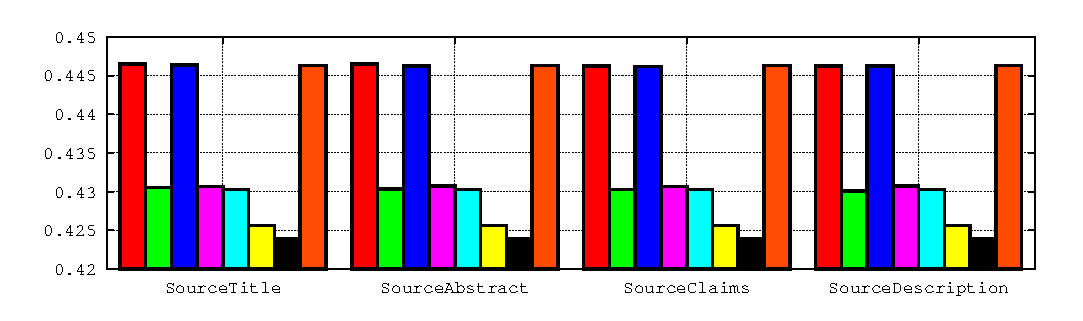
\includegraphics[width=5.5cm]{../Results-CIKM2014/qDescription-PRES-CLEF-IP2011}\label{fig:qDescription-PRES-CLEF-IP2011}} 
\par\end{centering}
%\caption{Patent Retrieval Evaluation Score (PRES) for QE methods on CLEF 2011 (for MMRQE $\lambda=0.5$).} \label{fig:PRES-CLEF2011}
\end{figure}

{\small *for MMRQE $\lambda=0.5$}
\end{frame}




\begin{frame}
\frametitle{MAP and PRES for QR methods on CLEF 2010}

\begin{figure}
\begin{centering}
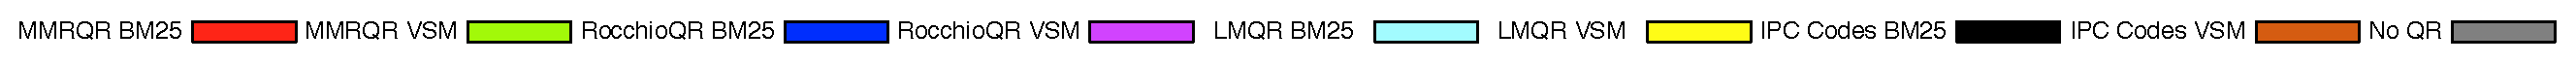
\includegraphics[width=10cm]{../img/legendQR}
\par\end{centering}

\begin{centering}
\subfigure[{Query Title.}]{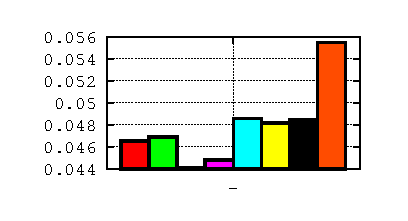
\includegraphics[width=2.5cm]{../mmrqrResults/qTitle-MAP-CLEF-IP2010}}\subfigure[{Query Abs.}]{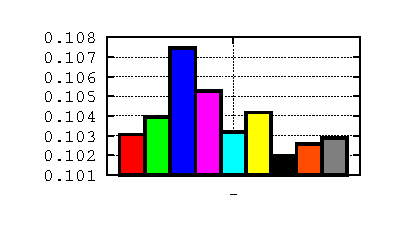
\includegraphics[width=2.5cm]{../mmrqrResults/qAbstract-MAP-CLEF-IP2010}}\subfigure[{Query Claims.}]{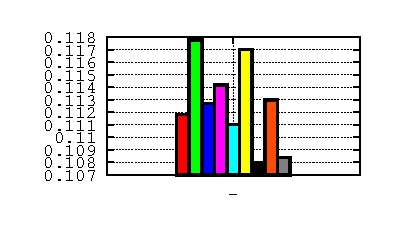
\includegraphics[width=2.5cm]{../mmrqrResults/qClaims-MAP-CLEF-IP2010}}
\subfigure[{Query Descr.}]{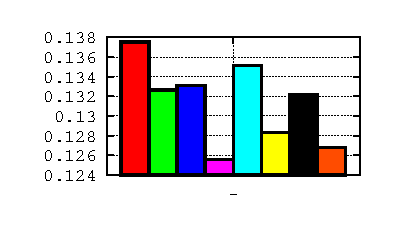
\includegraphics[width=2.5cm]{../mmrqrResults/qDescription-MAP-CLEF-IP2010}} 
\par\end{centering}
%\caption{Mean Average Precision (MAP) for QR methods on CLEF-IP 2010 (for MMRQR $\lambda=0.8$).} \label{fig:QR-PRES-CLEF-IP2010}
 \end{figure}


\begin{figure}
\begin{centering}
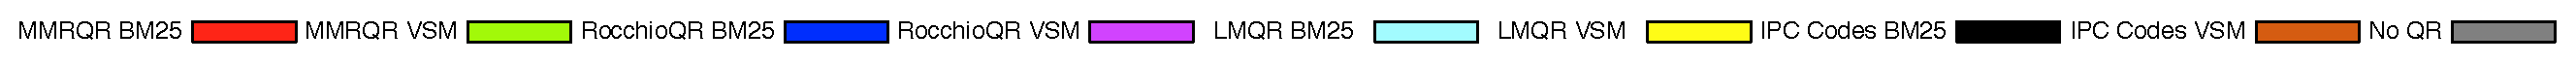
\includegraphics[width=10cm]{../img/legendQR}
\par\end{centering}

\begin{centering}
\subfigure[{Query Title.}]{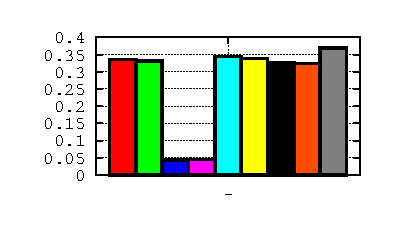
\includegraphics[width=2.5cm]{../mmrqrResults/qTitle-PRES-CLEF-IP2010}}\subfigure[{Query Abs.}]{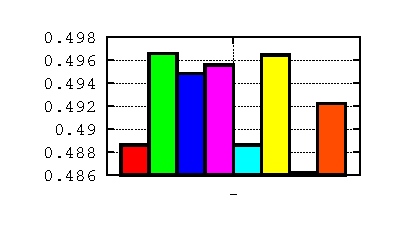
\includegraphics[width=2.5cm]{../mmrqrResults/qAbstract-PRES-CLEF-IP2010}}\subfigure[{Query Clai.}]{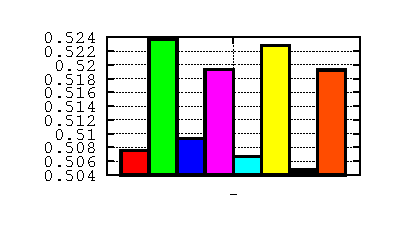
\includegraphics[width=2.5cm]{../mmrqrResults/qClaims-PRES-CLEF-IP2010}}
\subfigure[{Query Descr.}]{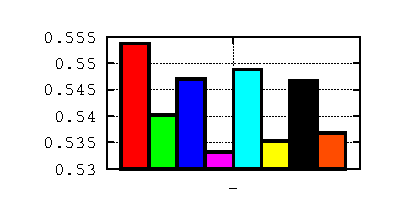
\includegraphics[width=2.5cm]{../mmrqrResults/qDescription-PRES-CLEF-IP2010}} 
\par\end{centering}
%\caption{Patent Retrieval Evaluation Score (PRES) for QR methods on CLEF 2010 (for MMRQR $\lambda=0.8$).} \label{fig:QR-MAP-CLEF-IP2010}
\end{figure}
{\small *for MMRQR $\lambda=0.8$}
\end{frame}



\begin{frame}
\frametitle{MAP and PRES for QR methods on CLEF 2011}

%\begin{figure}
%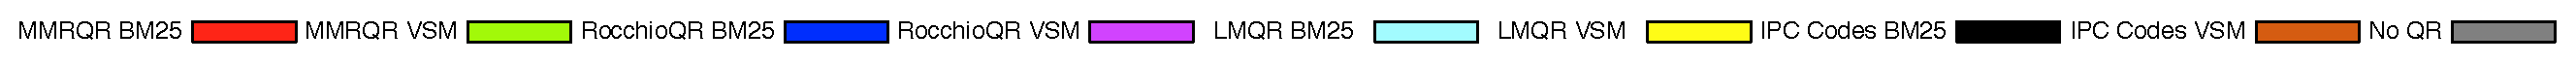
\includegraphics[width=10cm]{../img/legendQR}

%\subfigure[{Query Title.}]{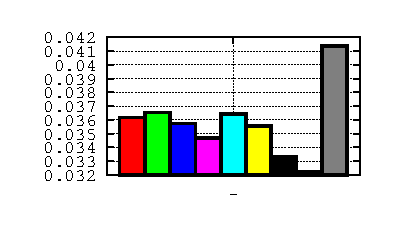
\includegraphics[width=2.5cm]{../mmrqrResults/qTitle-MAP-CLEF-IP2011}}\subfigure[{Query Abs.}]{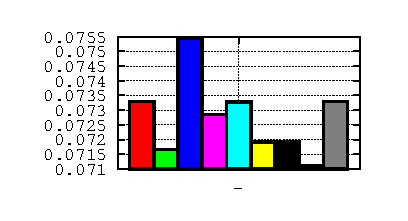
\includegraphics[width=2.5cm]{../mmrqrResults/qAbstract-MAP-CLEF-IP2011}}\subfigure[{Query Claims.}]{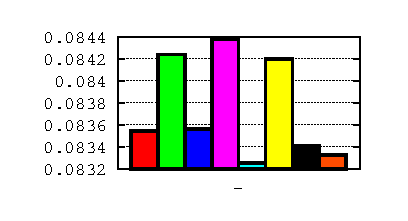
\includegraphics[width=2.5cm]{../mmrqrResults/qClaims-MAP-CLEF-IP2011}}
%\subfigure[{Query Descr.}]{\includegraphics[width=2.5cm]{../mmrqrResults/qDescription-MAP-CLEF-IP2011}} 

%\caption{Mean Average Precision (MAP) for QR methods on CLEF-IP 2011 (for MMRQR $\lambda=0.8$).} \label{fig:QR-PRES-CLEF-IP2011}
%\end{figure}

%\begin{figure}
%\includegraphics[width=10cm]{../img/legendQR}


%\begin{centering}
%\subfigure[{Query Title.}]{\includegraphics[width=2.5cm]{../mmrqrResults/qTitle-PRES-CLEF-IP2011}}\subfigure[{Query Abs.}]{\includegraphics[width=2.5cm]{../mmrqrResults/qAbstract-PRES-CLEF-IP2011}}\subfigure[{Query Claims.}]{\includegraphics[width=2.5cm]{../mmrqrResults/qClaims-PRES-CLEF-IP2011}}
%\subfigure[{Query Descr.}]{\includegraphics[width=2.5cm]{../mmrqrResults/qDescription-PRES-CLEF-IP2011}} \par\end{centering}
%\caption{Patent Retrieval Evaluation Score (PRES) for QR methods on CLEF 2011% (for MMRQR $\lambda=0.8$).}  \label{fig:QR-MAP-CLEF-IP2011}
%\end{figure}
%{\small *for MMRQR $\lambda=0.8$}
\end{frame}


\begin{frame}
\frametitle{}

Contributions are the following: 
\begin{enumerate}
\item Novel contributions for query expansion and reduction that leverage
(a) patent structure and (b) term diversification techniques. 
\item A thorough comparative analysis of existing and novel methods for
query expansion and reduction in patent prior-art search on standardized
datasets of CLEF-IP. 
\end{enumerate}
\end{frame}


\begin{frame}
\frametitle{}
\end{frame}

%\bibliographystyle{acl}
%\bibliography{biblio} 



\end{document}
